\ifdefined\MAINDOC\else
\documentclass[10pt, a4paper, fleqn]{article}
\usepackage{base}

\begin{document}
    \title{Skript Mathe 2}
    \date{06. Juni 2018} % Date here
    \maketitle
\fi

\subsection{Bemerkung}
Wähle $\delta = \dfrac{\epsilon}{k}$
\[
    \imp |f(x) - f(X_0)| \leq k \cdot |\underbrace{x - X_0}_{< \delta}| < k \cdot \delta = \epsilon \qed    
\]

\subsection{Beispiel}
\begin{enumerate}[a)]
    \item Anschauung zu 5.14a

    Es gibt 4 Fälle:

    \pgfplotsset{
        compat = 1.15,
        example axis/.style = {
            width = \textwidth,
            ytick = \empty, xtick = {10},
            xticklabels = {$X_0$},
            yticklabels = {$f(X_0)$},
            xmin = 0, xmax = 15,
            ymin = 0, ymax = 35,
            axis x line = center,
            axis y line = center,
            axis line style = {->},
            domain = 0:15
        },
        /pgf/declare function = {
            f141(\x) = -8.60*10^(-3)*x^4 
                +2.99*10^(-1)*x^3 
                -3.40*x^2 
                +12.61*x 
                +10;
        }
    }

    \begin{minipage}{0.4\textwidth}
        \begin{flushright}
            \begin{tikzpicture}
                \begin{axis}[
                    example axis,
                    ytick = {9}
                ]
                \draw[dashed] (10, 0) -- (10, 9) -- (0, 9);
                \addplot[color = black] {f141(x)};
                \draw (10, 9) node[circle, fill = black, scale = 0.3]{};
                \end{axis}
            \end{tikzpicture}
        \end{flushright}
    \end{minipage}
    \hfill
    \begin{minipage}{0.5\textwidth}
        $\lim\limits_{x \to X_0} f(x)$ existiert \\
        und ist gleich $f(x)$
    \end{minipage}

    \begin{minipage}{0.4\textwidth}
        \begin{flushright}
            \begin{tikzpicture}[
                declare function = {
                    g(\x) = f141(x) + 10;
                }
            ]
                \begin{axis}[example axis]
                \draw[dashed] (10, 0) -- (10, 19);
                \addplot[color = black, domain = 0:10] {f141(x)};
                \addplot[color = black, domain = 10:15] {g(x)};
                \end{axis}
            \end{tikzpicture}
        \end{flushright}
    \end{minipage}
    \hfill
    \begin{minipage}{0.5\textwidth}
        $\lim\limits_{x \to X_0} f(x)$ existiert nicht
    \end{minipage}

    \begin{minipage}{0.4\textwidth}
        \begin{flushright}
            \begin{tikzpicture}
                \begin{axis}[example axis, ytick = {27}]
                \draw[dashed] (10, 0) -- (10, 27) -- (0, 27);
                \addplot[color = black] {f141(x)};  
                \draw (10, 9) node[circle, draw = black, fill = white, scale = 0.5]{};
                \draw (10, 27) node[circle, fill = black, scale = 0.3]{};
                \end{axis}
            \end{tikzpicture}
        \end{flushright}
    \end{minipage}
    \hfill
    \begin{minipage}{0.5\textwidth}
        $\lim\limits_{x \to X_0} f(x)$ existiert \\
        und ist ungleich $f(X_0)$
    \end{minipage}

    \item Schule: $f$ ist stetig, wenn man $f$ ``ohne Absetzen'' zeichnen kann.

    Gegenbeispiel: $f:\IR \setminus \{0\} \to \IR, f(x) = \dfrac{1}{x}$ stetig
    auf $\IR \setminus \{0\}$

    \item Dirichlet--Funktion:
    \[f: \IR \to \IR, f(x) = \begin{cases}
        1 & x \in \IR \\
        0 & x \in \IR \setminus \IQ
    \end{cases}\]
    unstetig in jedem $X_0 \in \IR$.

    Mit $\epsilon$--$\delta$--Kriterium:

    Sei $\delta > 0$.
    \begin{enumerate}[1.]
        \item $X_0 \in \IQ \imp \ \exists x \in \IR \setminus \IQ: |x-X_0| < \delta$
        \item $X_0 \in \IR \setminus \IQ \imp \ \exists x \in \IR: |x-X_0| < \delta$
    \end{enumerate}
\end{enumerate}

\section*{Eigenschaften stetiger Funktionen}
\subsection{Satz: Rechenregeln für stetige Funktionen}

\begin{enumerate}[a)]
    \item Seien $f, g: D \to \IR$ stetig in $X_0 \in D, D \subseteq \IR, c \in \IR$. \\
    Dann sind auch $c \cdot f, f \pm g, f \cdot g$ und $ \dfrac{f}{g}$ 
    (für $g(x) \neq 0 \ \forall x \in D$) stetig.

    \item Seien $D, D' \subseteq \IR, f: D \to IR, g: D' \to \IR, f(D) \subseteq D'$. \\
    $f, g$ stetig $\imp g \circ f$ stetig.
\end{enumerate}

\textbf{Beweis: }
\begin{enumerate}[a)]
    \item Folgt direkt aus 5.14
    \item Mit 1.14 $\qed$
\end{enumerate}

\subsection{Bemerkung}
Wegen 5.16b und 5.20
\begin{enumerate}[a)]
    \item sind Monome und Polynome stetig
    \item Wegen a und 5.20a sind rationale Funktionen stetig
    \item Potenzreihen sind auf ihrem Konvergenzintervall stetig (zeigen wir hier nicht).
    Daher sind $\exp, \sin, \cos, \tan, \cotan$ (vgl. 3.11, 3.12) auch stetig.
\end{enumerate}

\subsection{Beispiele und Bemerkung zu Definitionslücken}
\begin{enumerate}[a)]
    \item Hebbare Definitionslücke:

    Sei $f: D \to \IR$ und $X_0$ HP von $X_0 \notin D$.
    Ist $\lim\limits_{x \to X_0} f(x) = a$, so heißt $X_0$
    stetig hebbare Definitionslücke von $f$.
    \[f: D \cup \{X_0\} \to \IR \quad \tilde{f}(x) = \begin{cases}
        f(x) & x \in D \\
        a & x = X_0
    \end{cases}\]
    heißt Fortsetzung von $f$ auf $D \cup \{X_0\}$.

    Beispiel: $f: \IR \setminus \{1\} \to \IR \quad f(x) = \dfrac{x^2 - 1}{x - 1}$
    \[
        \lim_{x \to 1} f(x) = \lim_{x \to 1} \frac{(x-1) \cdot (x+1)}{(x-1)} = 2    
    \]
    % TODO Graph?
    \[
        \tilde{f}: \IR \to \IR \quad \tilde{f}(x) = \begin{cases}
            f(x) & x \neq 1 \\
            2 & x = 1
        \end{cases} = x + 1
    \]

    \item Polstelle:

    Gilt für die Nullstelle $X_0$ des Nenners einer rationalen Funktion, dass
    $f(x) \to \pm \infty$, für $x \to X_0^-$ oder $x \to X_0^+$, so heißt $X_0$
    Polstelle.

    Beispiel: $f(x) = \dfrac{1}{x}$ hat Polstelle bei $X_0 = 0$.

    \item $f: \IR \setminus \{0\} \to \IR, f(x) = \sin\qt{\dfrac{1}{x}}$ hat in $X_0 = 0$ keinen Grenzwert.
 
    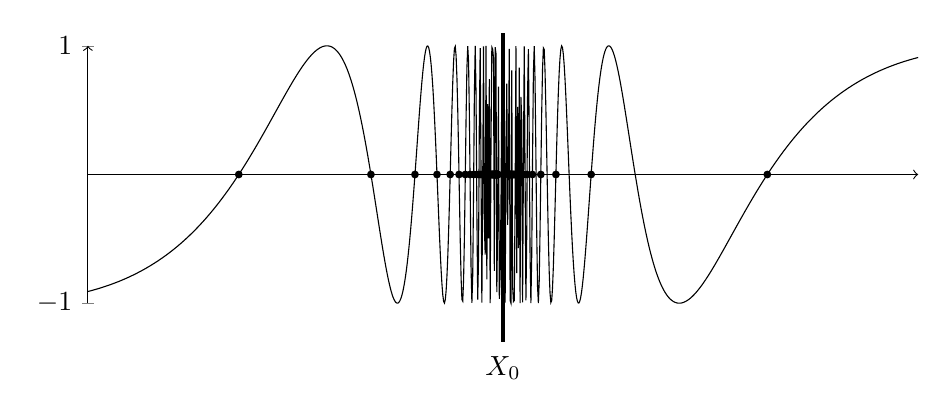
\begin{tikzpicture}
        \begin{axis}[
            width = \textwidth,
            height = 0.4\textwidth,
            xtick = {0}, ytick = {-1, 1},
            xticklabels = {$X_0$},
            ymin = -1, ymax = 1,
            axis x line = center,
            axis y line = left,
            axis line style = {->},
            domain = -0.5:0.5,
            xticklabel style = {yshift = -60pt},
            clip = false
        ]
         
        \foreach \k in {-1,...,-50,1,...,50} {
            \edef\tmp{\noexpand\draw ({1/(\k*pi)}, 0) node[circle, fill = black, scale = 0.3] {};}
            \tmp
        }
        \addplot[color = black, samples = 1000] {sin(deg(1/x))};
        \draw[line width = 0.5mm] (0, -1.3) -- (0, 1.1);
        \end{axis}

    \end{tikzpicture}

    Man nennt $X_0$ Oszillationsstelle:
    \begin{itemize}
        \item $X_n = \dfrac{1}{n \pi} \to 0$ und $f(X_n) = \sin(n \pi) = 0$
        \item $Y_n = \dfrac{1}{n \cdot 2 \pi + \frac{\pi}{2}} \to 0$ und $f(Y_n) = \sin(2 \pi n + \frac{\pi}{2}) = 1$
    \end{itemize}
    \[\begin{aligned}
        &\imp f(Y_n) \to 1 \\
        &\imp \lim_{x \to 0} f(x) \text{ existiert nicht.}
    \end{aligned}\]

    \item $f: \IR \setminus \{0\} \to \IR \quad f(x) = x \cdot \sin\qt{\dfrac{1}{x}}$
    hat in $X_0 = 0$ \\ 
    eine hebbare Definitionslücke

    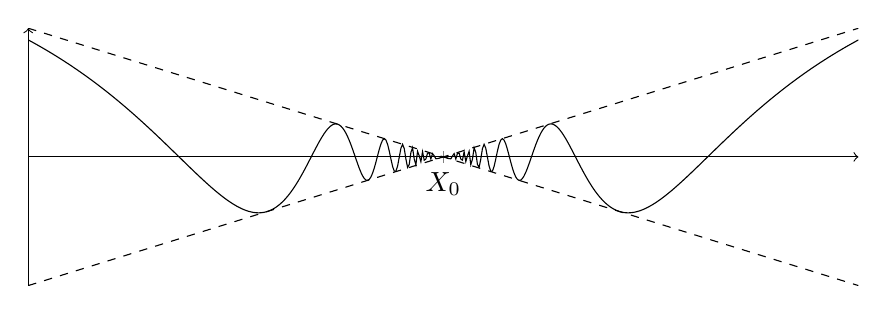
\begin{tikzpicture}
        \begin{axis}[
            width = \textwidth,
            height = 0.4\textwidth,
            xtick = {0}, ytick = \empty,
            xticklabels = {$X_0$},
            ymin = -0.5, ymax = 0.5,
            axis x line = center,
            axis y line = left,
            axis line style = {->},
            domain = -0.5:0.5,
        ]
         
        \addplot[color = black, samples = 500] {x*sin(deg(1/x))};
        \addplot[color = black, dashed] {x};
        \addplot[color = black, dashed] {-x};
        \end{axis}
    \end{tikzpicture}
        
    $f(X_n) = \underbrace{X_n}_{\to 0} \cdot \underbrace{\sin\qt{\frac{1}{X_n}}}_{\text{beschränkt}}$
    für jede Nullfolge $(X_n)$ in $\IR \setminus \{0\}$

    $
        \imp \tilde{f}(x) = \begin{cases}
            x \cdot \sin\qt{\frac{1}{x}} & x \neq 0 \\
            0 & x = 0
        \end{cases}    
    $ stetige Fortsetzung.

    \item $f: \IR \setminus \{0\} \to \IR \quad f(x) = \sin(x) \cdot \frac{1}{x}$
    
    Wir zeigen später mit L'Hopital, dass $\lim\limits_{x \to 0} f(x) = 1$

\end{enumerate}

\subsection{Satz: Zwischenwertsatz von Bolzano (Nullstellensatz)}

$f: [a, b] \to \IR$ stetig, $f(a) \cdot f(b) < 0$.
Dann: Es gibt $c \in [a, b]$ mit $f(c) = 0$.

\textbf{Beweis: }
$f(a) \cdot f(b) < 0$ bedeutet, dass $f(a)$ und $f(b)$ unterschiedliche Vorzeichen haben.

Beweis für $f(a) < 0, f(b) > 0$ (Anderer Fall analog)

Anschaulich klar, da $f$ keine Sprungstelle hat.

\textbf{Bisektionsverfahren: }

Start $[a_1, b_1] := [a, b]$

1. Schritt: Halbiere $[a_1, b_1]$
\begin{itemize}
    \item Berechne $y_1 = f\qt{\frac{a_1 + b_1}{2}}$
    \item Fallunterscheidung:
    \begin{itemize}
        \item $y_1 = 0$: Fertig
        \item $y_1 > 0$:
            Neues Intervall $[a_2, b_2] := [a_1, \frac{a_1 + b_1}{2}]$
        \item $y_1 < 0$:
            Neues Intervall $[a_2, b_2] := [frac{a_1 + b_1}{2}, b_1]$
    \end{itemize}
    \item Es gilt:
    \begin{itemize}
        \item $[a_2, b_2]$ halb so groß wie $[a_1, b_1]$
        \item $f(a_2) < 0, f(b_2) > 0$
    \end{itemize}
\end{itemize}
2. Schritt: Wende Schritt 1 auf $[a_2, b_2]$ an, erhalte $y_2$ und $[a_3, b_3]$

Usw...


\ifdefined\MAINDOC\else
\end{document}
\fi